\begin{figure*}[hbtp]
  \centering
  % \includegraphics[width=0.44\linewidth]{out/insertions-speedup-key.pdf}
  \subfigure[Overall result]{
    \label{fig:insertions-speedup--mean}
    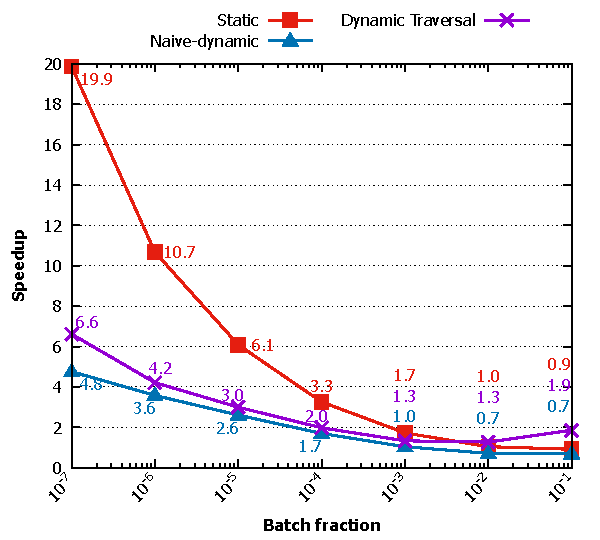
\includegraphics[width=0.38\linewidth]{out/insertions-speedup-mean.pdf}
  }
  \subfigure[Results on each graph]{
    \label{fig:insertions-speedup--all}
    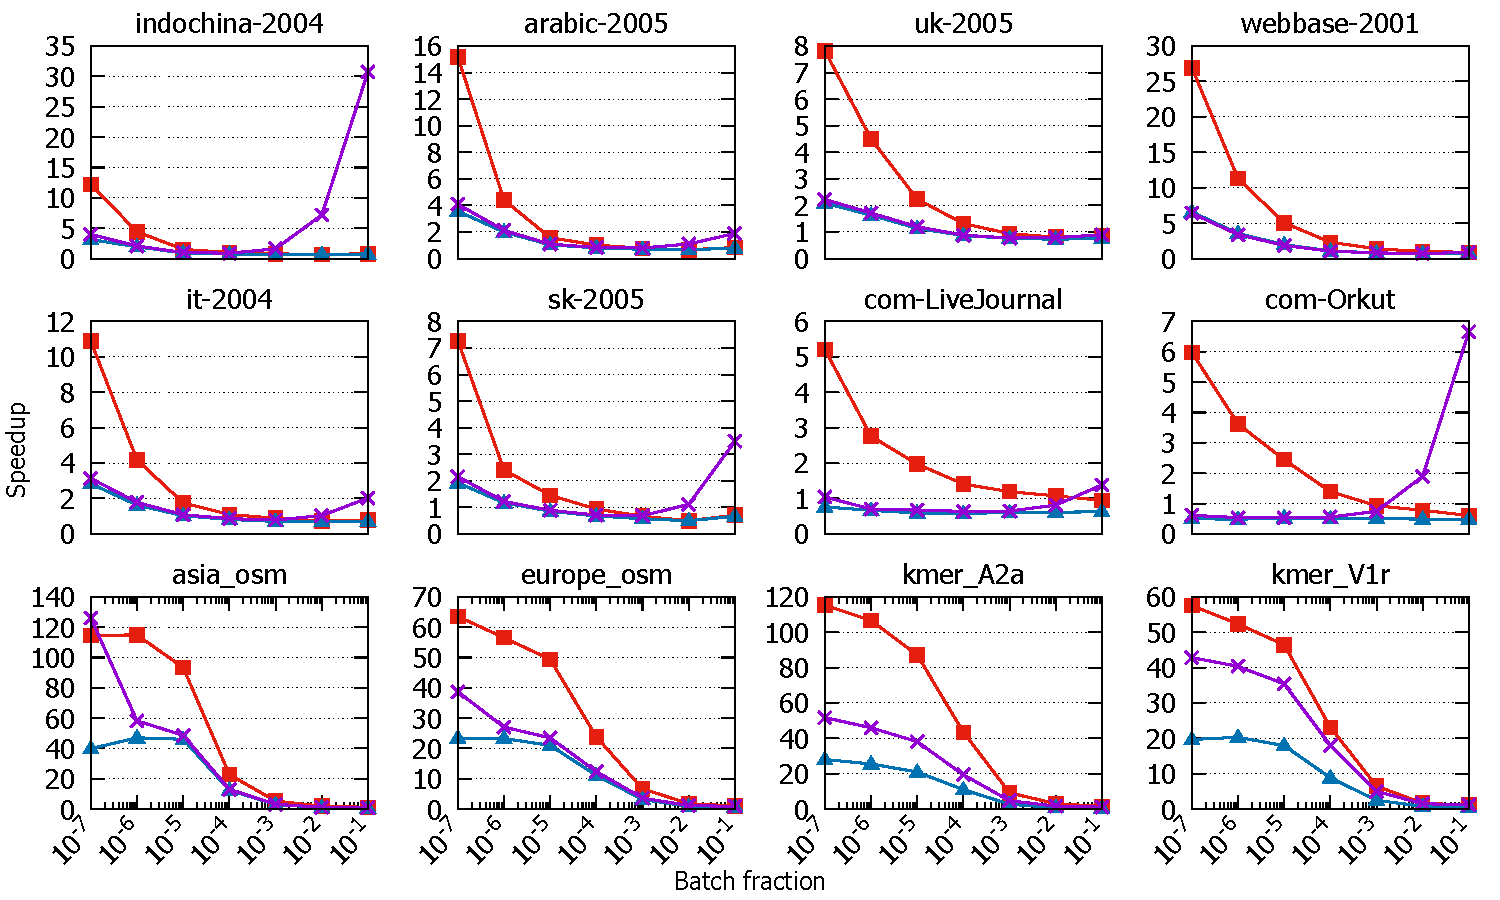
\includegraphics[width=0.58\linewidth]{out/insertions-speedup-all.pdf}
  } \\[-1ex]
  \caption{Insertions Time taken (solid lines), and modularity of communities obtained (dashed lines) along the Y2 axis, with X, X, and X (Algorithm X) on batch updates of increasing size from $10^{-7} |E|$ to $0.1 |E|$. Note that both axes are logarithmic. The numbers on the lines corresponding to X and X indicate the speedup of X over  the two algorithms, respectively.}
  \label{fig:insertions-speedup}
\end{figure*}
